\documentclass[10pt,english,aspectratio=169]{beamer}
% Use notes or hide notes or show only notes or handout

\usetheme{default}

\usepackage{xstring}
\usepackage{pgfpages}
%\makeatletter
%\IfSubStr{\@classoptionslist}{handout}
%  {\pgfpagesuselayout{2 on 1}[letterpaper,border shrink=5mm]}
%  {}
%\makeatother

\usepackage{amsmath,amssymb,amsthm}
\usepackage{stmaryrd}
\usepackage{enumerate}
\usepackage{stfloats}
\usepackage{bbm}
\usepackage{pdfpages}
\usepackage{framed}

\usepackage[most]{tcolorbox}
\tcbset{highlight math style={enhanced,
  colframe=white,colback=yellow!15,arc=8pt,boxrule=1pt,
  }}
  
\usepackage{tikz,pgf,pgfplots}
\usepackage{algorithm,algorithmic}
\usepgflibrary{shapes}
\usetikzlibrary{%
  automata,%
  arrows,%
  arrows.meta,
  backgrounds,
  shapes.misc,% wg. rounded rectangle
  shapes.arrows,%
  shapes,%
  calc,%
  chains,%
  matrix,%
  positioning,% wg. " of "
  scopes,%
  decorations.pathmorphing,% /pgf/decoration/random steps | erste Graphik
  shadows,%
  backgrounds,%
  fit,%
  petri,%
  quotes
}

\tikzset{background rectangle/.style={
    fill=white,
  },
  use background/.style={    
    show background rectangle
  }
}

\setbeamersize{text margin left=10mm,text margin right=35mm}

\pgfplotsset{compat=1.12}

%\usetheme{Frankfurt}
%\usecolortheme{ldpc}
\useinnertheme{rounded}
\usecolortheme{whale}
\usecolortheme{orchid}

\newcommand{\ul}[1]{\underline{#1}}
\renewcommand{\Pr}{\mathbb{P}}

%% Setup slides and notes
\makeatletter
\IfSubStr{\@classoptionslist}{notes} { \IfSubStr{\@classoptionslist}{hide} {}{\IfSubStr{\@classoptionslist}{only} {}{\setbeameroption{show notes on second screen=right}}} }{}
\makeatother
%\setbeamertemplate{note page}{\pagecolor{yellow!5}\vfill\insertnote\vfill}

\newcommand{\getpdfpages}[2]{\begingroup
  \setbeamercolor{background canvas}{bg=}
  \addtocounter{framenumber}{1}
  \includepdf[pages={#1},%
  pagecommand={%
    \expandafter\def\expandafter\insertshorttitle\expandafter{%
      \insertshorttitle\hfill\insertframenumber\,/\,\inserttotalframenumber}}%
  ]{#2}
  \endgroup}

\newcommand{\backupbegin}{
   \newcounter{finalframe}
   \setcounter{finalframe}{\value{framenumber}}
}
\newcommand{\backupend}{
   \setcounter{framenumber}{\value{finalframe}}
}

 \setbeamercolor{bibliography entry author}{fg=black}
 \setbeamercolor{bibliography entry title}{fg=black}
 \setbeamercolor{bibliography entry location}{fg=black}
 \setbeamercolor{bibliography entry note}{fg=black}
 
 \setbeamerfont{bibliography item}{size=\footnotesize}
 \setbeamerfont{bibliography entry author}{size=\footnotesize}
 \setbeamerfont{bibliography entry title}{size=\footnotesize}
 \setbeamerfont{bibliography entry location}{size=\footnotesize}
 \setbeamerfont{bibliography entry note}{size=\footnotesize}
 \setbeamertemplate{bibliography item}{\insertbiblabel}
 
\newlength\tikzwidth
\newlength\tikzheight


\newcommand{\mc}[1]{\mathcal{#1}}
\newcommand{\mbb}[1]{\mathbb{#1}}
%\newcommand{\expt}{\mbb{E}}
%\newcommand{\dd}{\mathrm{d}}
\newcommand{\Interior}[1]{\ensuremath{{#1}^{\circ}}}
\newcommand{\Closure}[1]{\ensuremath{\overline{#1}}}
\newcommand{\Complement}[1]{\ensuremath{{#1}^{c}}}

\newcommand{\Expect}{\ensuremath{\mathrm{E}}}
\newcommand{\vecnot}{\underline}
\newcommand{\RealNumbers}{\ensuremath{\mathbb{R}}}
\newcommand{\RationalNumbers}{\mathbb{Q}}
\newcommand{\ComplexNumbers}{\mathbb{C}}
\newcommand{\Real}{\mathrm{Re}}
\newcommand{\Span}{\mathrm{span}}
\newcommand{\Rank}{\mathrm{rank}}
\newcommand{\Nullity}{\mathrm{nullity}}
\newcommand{\Trace}{\mathrm{tr}}
\newcommand{\Diag}{\mathrm{diag}}
\newcommand{\dd}{\mathrm{d}}
\DeclareMathOperator*{\esssup}{ess\,sup}

% Use < , > inner product
\newcommand{\inner}[2]{{\left\langle #1 \mskip2mu , #2 \right\rangle}}
\newcommand{\tinner}[2]{{\langle #1 \mskip1mu , #2 \rangle}}

% Use < | > inner product
%\newcommand{\inner}[2]{{\left\langle #1 \mskip2mu \middle| \mskip2mu #2 \right\rangle}}
%\newcommand{\tinner}[2]{{\langle #1 \mskip1mu | \mskip1mu  #2 \rangle}}




\def\checkmark{\tikz\fill[scale=0.4](0,.35) -- (.25,0) -- (1,.7) -- (.25,.15) -- cycle;}
\def\greencheck{{\color{green}\checkmark}}
\def\scalecheck{\resizebox{\widthof{\checkmark}*\ratio{\widthof{x}}{\widthof{\normalsize x}}}{!}{\checkmark}}
\def\xmark{\tikz [x=1.4ex,y=1.4ex,line width=.2ex, red] \draw (0,0) -- (1,1) (0,1) -- (1,0);}
\def\redx{{\color{red}\xmark}}

\renewcommand{\footnotesep}{-2pt}


\begin{document}

\title{ECE 586: Vector Space Methods \\ Lecture 12 Flip Video: Markov Chains}
\author{Henry D. Pfister \\ Duke University}
\date{}
%\date{August 20th, 2020}
%\maketitle

\setbeamertemplate{navigation symbols}{}

\begin{frame}[plain]
	\titlepage
	
	\note{
		\vspace{8mm}
		\begin{enumerate}
			\setlength\itemsep{3mm}
			\color{red}
			\item Welcome to the 12th video lecture for ECE 586, Vector Space Methods. \\[2mm]
			Today, we'll discuss Markov chains as an application of linear transforms.
		\end{enumerate}
	}
\end{frame}

\addtocounter{framenumber}{-1}
\setbeamertemplate{navigation symbols}{\textcolor{blue}{\footnotesize \insertframenumber ~/ \inserttotalframenumber}}


\begin{frame}<1-2> \frametitle{Chutes and Ladders}

\vspace{-3mm}

\begin{center}
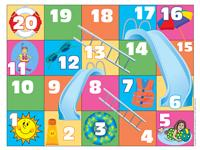
\includegraphics[scale=0.9]{minichutes.jpg}
\end{center}
\vspace{-4mm}

\begin{example}<1-> [Chutes and Ladders or Snakes and Ladders]
 is a boardgame where a single die is rolled to determine how far you move on a gameboard defined by a grid. Some locations contain ladders that let you skip ahead while others contains chutes (or snakes) that set you back. It is based on an ancient game from India that teaches morality by associating ladders with virtues and snakes with vices.
\end{example}

\uncover<2->{\textcolor{red}{Q: What is the chance a player finishes the game in $m$ or fewer moves?}}

\vspace{-1mm}

\note{
	\vspace{2mm}
	\begin{enumerate}[<alert@+>]
		\footnotesize
		\setlength\itemsep{3mm}
		\item Read.
		\item Read.
	\end{enumerate}
}

\end{frame}

\begin{frame}<1-4> \frametitle{Markov Chains}

\begin{definition}<1->
A \textcolor{blue}{finite-state Markov chain (FSMC)} with $n$ states is a sequence of random variables $X_{1},X_{2},X_{3},\ldots$ where each $X_{i}\in[n]\triangleq\left\{ 1,2,\ldots,n\right\} $ and \vspace{-2mm}
\[
\Pr\left(X_{t+1}=j\,\middle|\,X_{t}=i,X_{1},X_{2},\ldots,X_{t-1}\right)=\Pr\left(X_{t+1}=j\,\middle|\,X_{t}=i\right).
\]
\end{definition}

\begin{definition}<2->
If $\Pr(X_{t+1}=j\,|\,X_{t}=i)$ does not depend on $t$, then the Markov chain\\ is called \textcolor{blue}{time invariant}.
For a time-invariant FSMC, let $P\in\mathbb{R}^{n\times n}$\\ denote the \textcolor{blue}{transition probability matrix} with entries
\[\left[P\right]_{i,j}\triangleq P_{i,j}=\Pr(X_{t+1}=j\,|\,X_{t}=i).\]
\end{definition}

\vspace{2mm}

\uncover<3->{Since each row of $P$ is a probability distribution, $P_{i,j}\geq0$ and\\ $\sum_{j=1}^{n}P_{i,j}=1$.  Matrices with this property are called \textcolor{blue}{stochastic}}

\uncover<4->{%
\begin{tikzpicture}[overlay,remember picture,shift={(10.75,1.0)},->, >=stealth', auto, semithick, node distance=3cm]

\draw[fill=yellow!20,rounded corners] (-0.2,-0.9) rectangle (4.0,2.6);

	\tikzstyle{every state}=[fill=white,draw=black,thick,text=black,scale=0.6]
	\node[state]    (A) at (0.87,-0.25)                   {$1$};
	\node[state]    (B)[above of=A]   {$2$};
	\node[state]    (C)[right of=B]   {$3$};
	\node[state]    (D)[below of=C]   {$4$};
	\path
	(A) edge[loop right]			node{$2/3$}	(A)
	(B) edge[left,<-]	node{$1/3$}	(A)
	edge[bend left,above]		node{$1$}	(C)
	(C) edge[bend left,below]	node{$2/3$}	(B)
	edge[right]		node{$1/3$}	(D)
	(D) edge[loop right]		node{$1$}	(D);

\end{tikzpicture}
}

\note{
	\vspace{2mm}
	\begin{enumerate}[<alert@+>]
		\footnotesize
		\setlength\itemsep{3mm}
		\item Read.
		\item Read.
		\item Read.
		\item Read.
	\end{enumerate}
}


\end{frame}

\begin{frame}<1-2> \frametitle{Properties of Time-Invariant Markov Chains}

\vspace{-1.5mm}

\begin{exampleblock}{Multiple-Step Transition Probability}<1->
\vspace{-4mm}
\begin{align*}
\Pr\left(X_{t+2}=j\,\middle|\,X_{t}=i\right) & =\sum_{k=1}^{n}\Pr\left(X_{t+2}=j\,\middle|\,X_{t+1}=k\right)\Pr\left(X_{t+1}=k\,\middle|\,X_{t}=i\right)\\
 & =\sum_{k=1}^{n}P_{k,j}P_{i,k}=\sum_{k=1}^{n}P_{i,k}P_{k,j}=\left[P^{2}\right]_{i,j}
\end{align*}
By induction, it follows that $\Pr(X_{t+m}=j\,|\,X_{t}=i)=\left[P^{m}\right]_{i,j}$.
\end{exampleblock}
\vspace{-0.5mm}
\begin{exampleblock}{Matrix-Vector Notation}<2->
Using the notation $\vecnot{\pi}^{(t)}=(\pi_{1}^{(t)},\ldots,\pi_{n}^{(t)})$ with $\pi_{i}^{(t)}\triangleq\Pr(X_{t}=i)$, we see that \vspace{-2.5mm}
\begin{align*}
\pi_{j}^{(t+1)} & =\sum_{i=1}^{n}\Pr(X_{t+1}=j,X_{t}=i) 
=\sum_{i=1}^{n}\Pr(X_{t+1}=j|X_{t}=i)\Pr(X_{t}=i)\\
 & =\sum_{i=1}^{n}P_{i,j}\pi_{i}^{(t)}=\left[\vecnot{\pi}^{(t)}P\right]_{j}=\left[\vecnot{\pi}^{(t-1)}P^2\right]_{j}= \cdots = \left[\vecnot{\pi}^{(1)}P^t\right]_{j}.%, \quad \text{where} \; \; \pi_{i}^{(1)} = \Pr(X_1 = i)
 \vspace*{-0.5mm}
\end{align*}
\end{exampleblock}

\note{
	\vspace{2mm}
	\begin{enumerate}[<alert@+>]
		\footnotesize
		\setlength\itemsep{3mm}
		\item Read.
		\item Read.
	\end{enumerate}
}

\end{frame}

\begin{frame} \frametitle{Simulating a Markov Chain}

Let the random variable $U$ be uniformly distributed on the interval $[0,1)$.
To simulate a discrete random variable $X\in[n]$, one can use $U$ to simulate $X$ by assigning subintervals of $[0,1)$ to each of the $n$ possibilities for $X$. \\ [4mm]

Let $F_{X}(x)=\sum_{i=1}^{x}\Pr(X=i)$ for $x\in[n]$ be the cumulative distribution function of $X$. Then, one can set $X=x$ if $U\in[F_{X}(x-1),F_{X}(x))$ (with $F_{X}(0)=0$ by convention). This works because 
\[
\Pr \Big( U\in \big[F_{X}(x-1),F_{X}(x) \big) \Big)=F_{X}(x)-F_{X}(x-1)=\Pr(X=x).
\]
\\

\uncover<2->{Using this, one can simulate a Markov chain by using pseudo-random numbers to generate realizations of the process.
If $X_t = x$, then $X_{t+1} = x'$ is generated according to $\Pr(X_{t+1}=x'|X_t = x)$ using the above method.}

\note{
	\vspace{2mm}
	\begin{enumerate}[<alert@+>]
		\footnotesize
		\setlength\itemsep{3mm}
		\item Read.
		\item Read.
	\end{enumerate}
}

\end{frame}

\begin{frame}<1-3> \frametitle{Hitting Time}

\begin{definition}For a Markov chain starting from state $i$, the first \textcolor{blue}{hitting time} of state $j$ is a random variable $T_{i,j}$ with distribution \vspace{-2mm}
\[
\Pr\left(T_{i,j}=m\right)=\Pr\left(X_{m+1}=j,X_{m}\neq j,X_{m-1}\neq j,\ldots,X_{2}\neq j\,\middle|\,X_{1}=i\right)
\]
and, by convention, $\Pr\big(T_{i,j}=0\big)=\delta_{i,j}$ where $\delta_{i,j}$ is Kronecker delta function. If state $j$ is not reachable from state $i$, then $T_{i,j} = \infty$ by convention.
\end{definition}

\begin{definition}<2->
If the process can become stuck in state $j$ (i.e., $P_{j,j} = 1$), then state $j$ is called \textcolor{blue}{absorbing}.
\end{definition}

\begin{exampleblock}{Lemma}<3->
If state $j$ is absorbing, then the distribution of the hitting time $T_{i,j}$ satisfies \vspace{-2mm}
\[
\Pr\left(T_{i,j}\leq m\right)=\Pr\left(X_{m+1}=j\,\middle|\,X_{1}=i\right)=\left[P^{m}\right]_{i,j}.
\]
\end{exampleblock}

\note{
	\vspace{2mm}
	\begin{enumerate}[<alert@+>]
		\footnotesize
		\setlength\itemsep{3mm}
		\item Read.
		\item Read.
		\item Read.
	\end{enumerate}
}

\end{frame}

\begin{frame}<1-5> \frametitle{Stationary Probabilities of Recurrent Markov Chains}

\begin{definition}<1->
A state distribution $\vecnot{\pi}$ is called \textcolor{blue}{stationary} if it satisfies $\vecnot{\pi}P=\vecnot{\pi}$.
\end{definition}

\begin{definition}<2->
State $j$ is \textcolor{blue}{reachable} from state $i$ if $[P^m]_{i,j} >0$ for some $m\in \mathbb{N}$.
Two states reachable from each other are \textcolor{blue}{communicating}.
A state is \textcolor{blue}{recurrent} if it is expected to return to itself infinitely many times.
%If all pairs of states are communicating, the chain is \textcolor{blue}{irreducible} and all states are recurrent.

\end{definition}

\begin{exampleblock}{Theorem (Perron)}<3->
If $P_{i,j}>0$ for all $i,j\in[n]$, then every state is recurrent and the Markov chain has a unique stationary distribution. This also holds if all entries of $P^m$ are strictly positive for some $m\geq 1$. The stationary distribution $\vecnot{\pi}$ equals the expected fraction of time that the process spends in each state.
\end{exampleblock}

\uncover<4->{Can find stationary distribution using row reduction after rewriting $\vecnot{\pi}P=\vecnot{\pi}$ as \vspace{0mm}
\[
(I-P)^{T}\vecnot{\pi}^{T}=\vecnot 0.
\]}

\uncover<5->{%
\begin{tikzpicture}[overlay,remember picture,shift={(10.75,1.0)},->, >=stealth', auto, semithick, node distance=3cm]

\draw[fill=yellow!20,rounded corners] (1.2,0.2) rectangle (3.9,3.8);

	\tikzstyle{every state}=[fill=white,draw=black,thick,text=black,scale=0.6]
	\node[state]    (A) at (2.5,1.2)                   {$1$};
	\node[state]    (B) at (2.5,2.7) {$2$};
	\path
	(A) edge[loop below,right]			node{$2/3$}	(A)
	(B) edge[loop above,right]	node{$1/3$}	(B);
    \path
    (A) edge[bend left,left]		node{$1/3$}	(B);
    \path
    (B) edge[bend left,right]		node{$2/3$}	(A);

\end{tikzpicture}
}

\note{
	\vspace{2mm}
	\begin{enumerate}[<alert@+>]
		\footnotesize
		\setlength\itemsep{3mm}
		\item Read.
		\item Read.
		\item Read.
		\item Read.		
		\item Read.		
	\end{enumerate}
}

\end{frame}


\begin{frame} \frametitle{Next Steps}

\begin{itemize}
\setlength\itemsep{5mm}
\item To continue studying after this video -- \vspace{2mm}

\begin{itemize}
 \setlength\itemsep{3mm}
 \item Try the required reading: Markov Chains Handout
\end{itemize}
\end{itemize}

\note{
	\vspace{8mm}
	\begin{enumerate}
		\setlength\itemsep{3mm}
		\color{red}
		\item Here are some options to continue learning this material. (read) \\ [2mm]  That's it for today.  So, I'll see you next time.
	\end{enumerate}
}

\end{frame}


\backupbegin

%\begin{frame}
%\frametitle{Backup Slides}
%\begin{itemize}
%\item Slide numbers not included in denominator!
%\end{itemize}
%\end{frame}

%\begin{frame}[allowframebreaks]
%\frametitle{References}
%\bibliographystyle{alpha}
%\footnotesize
%\bibliography{IEEEabrv,WCLabrv,WCLbib,WCLnewbib}
%\end{frame}

\backupend

\end{document}
